\section{Evaluation}\label{sec:eval}

Our prototype implementation is available on \href{https://github.com/AurelienCha/Decentralized-Sphinx}{GitHub}\footnote{\url{https://github.com/AurelienCha/Decentralized-Sphinx}}.
The implementation is written in Python 3.13 using the ECPy library for elliptic curve operations. 
ECPy is well-suited for prototyping due to its simplicity, but it is significantly slower than many EC python libraries (approximately one order of magnitude slower). 
Nevertheless, it remains one of the few Python libraries supporting Montgomery Curve25519, which is essential for our implementation.

We evaluate our system on two main axes: computational complexity and unlinkability (i.e. resistance to correlation between incoming and outgoing packets).

\subsection{Computational Complexity}

Instead of measuring raw execution time, which can vary significantly based on hardware and software environments, we focus on the number of expensive cryptographic operations. 
Table \ref{tab:operation_count} count these operations per party for $ m $ TTPs and path of length $ p $. 
To compute the total cost for sending one message, the TTP cost should be multiplied by $ m $ and the mixnode cost by $ p $.

\begin{table}[h]
    \begin{tabularx}{0.9\textwidth} { 
        l
    | >{\centering\arraybackslash}X 
    | >{\centering\arraybackslash}X 
    | >{\centering\arraybackslash}X 
    | >{\centering\arraybackslash}X  }
        & \textbf{Client} & \textbf{TTP} & \textbf{Mixnode} \\
        \hline
        \textbf{EC Multiplication}              & \bigO{p \, m} & \bigO{p^{2}} & \bigO{p} \\
        \textbf{EC Addition}                    & \bigO{p \, m} & \bigO{p^{2}} & \bigO{p} \\
        \textbf{Point $\rightarrow$ Integer}    & \bigO{p} & 0 & 2 \\
        \textbf{Integer $\rightarrow$ Point}    & \bigO{p} & 0 & 0 \\
    \end{tabularx}
    \label{tab:operation_count}
    \newline
    \caption{Number of expensive cryptographic operations per party, where $ p $ is the path length (e.g. $ p = 3 $), and $ m $ is the number of TTPs.}
\end{table}
% NOTE: Precision version
% \begin{table}
%     \begin{tabularx}{0.9\textwidth} { 
%         l
%     | >{\centering\arraybackslash}X 
%     | >{\centering\arraybackslash}X 
%     | >{\centering\arraybackslash}X 
%     | >{\centering\arraybackslash}X  }
%         & \textbf{Client} & \textbf{TTP} & \textbf{Mixnode} \\
%         \hline
%         \textbf{EC Multiplication}              & $ p (m+1) $   & $ 3 p^2 - 3 p + 2 $   & $ 2 p + 4$ \\
%         \textbf{EC Addition}                    & $ 3 p (m-1) $ & $ 5 p^2 - 7 p + 4 $   & $ 4 p $ \\
%         \textbf{Point $\rightarrow$ Integer}    & $ p $         & $ 0 $                 & $ 2 $ \\
%         \textbf{Integer $\rightarrow$ Point}    & $ p $         & $ 0 $                 & $ 0 $ \\
%     \end{tabularx}
%     \label{tab:operation_count}
%     \newline
%     \caption{\vspace*{5mm} TODO: p = path size (3) and, m is nbr of TTP (3)}
% \end{table}

Since long paths are typically unnecessary, we can approximate \bigO{p} as constant (i.e. \bigO{1}). 
A path of length $ p = 3 $ is generally sufficient to ensure strong anonymity. \todo{Aurelien: Iness do you have some source to support this ? If yes, could you cite here, thanks.}
Consequently, the overall computational burden is more sensitive to the number of TTPs $ m $ rather than the path length. 
Because our design remains secure as long as a single TTP is honest (i.e. does not collude), only a small number of TTPs may be required. 
A deeper analysis of how many TTPs are needed to ensure a desired level of trust remains an open question for future work.


\subsection{Unlinkability assessment}

Quantifying unlinkability is inherently challenging. 
However, under the assumption that uniformly random packet headers prevent adversaries from correlating incoming and outgoing packets via cryptanalysis, 
unlinkability can be approximated by assessing the statistical randomness of the headers.

We rely on the NIST SP 800-22 statistical test suite \cite{NIST-SP80022}, which includes 15 tests designed to assess the quality of random number generators. 
Each test returns a p-value representing how likely the data could be produced by a uniform source. 
If the outputs are truly random, the distribution of p-values across many samples should itself be uniform.

\todo[inline,color=blue!30]{Add a brief description of these tests (i.e. what is evaluating) -> no, too long (or for appendix)}
\todo{TODO: For the moment, only the first 4 of the 15 NIST tests have been implemented.}


For our prototype, we simulate a network of 20 mixnodes and 3 TTPs.\newline 
At each iteration:
\begin{itemize}
    \item A random destination IP and path of 3 mixnodes are selected;
    \item The client generates shares and distributes them to the three TTPs;
    \item TTPs independently compute partial headers, which are then aggregated and forwarded through the simulated mixnet.
\end{itemize}

Each run produces 4 headers (one per hop).
We perform 100 000 runs, resulting in a 400 000 x 1792 matrix (400 000 headers of 1792 bits).
Then we apply the NIST tests to each:
\begin{itemize}
    \item header independently (i.e. row-wise) to obtain p-value distributions across headers (Figure \ref{fig:sp_800-22_hist_headerwise}).
    \item bit independently (i.e. column-wise) to ensure no bias exists in specific bit positions (Figure \ref{fig:sp_800-22_hist_bitwise}).
\end{itemize}

For comparison, we conduct the same evaluation on the original Sphinx implementation by Danezis\footnote{\href{https://github.com/UCL-InfoSec/sphinx}{https://github.com/UCL-InfoSec/sphinx}}, which produces 400 000 headers of 1634 bits. 
Figures \ref{fig:sp_800-22_hist_headerwise} and \ref{fig:sp_800-22_hist_bitwise} compare header randomness of our implementation (in orange) with the original implementation (in blue).
\begin{figure}[H]
    \centering
    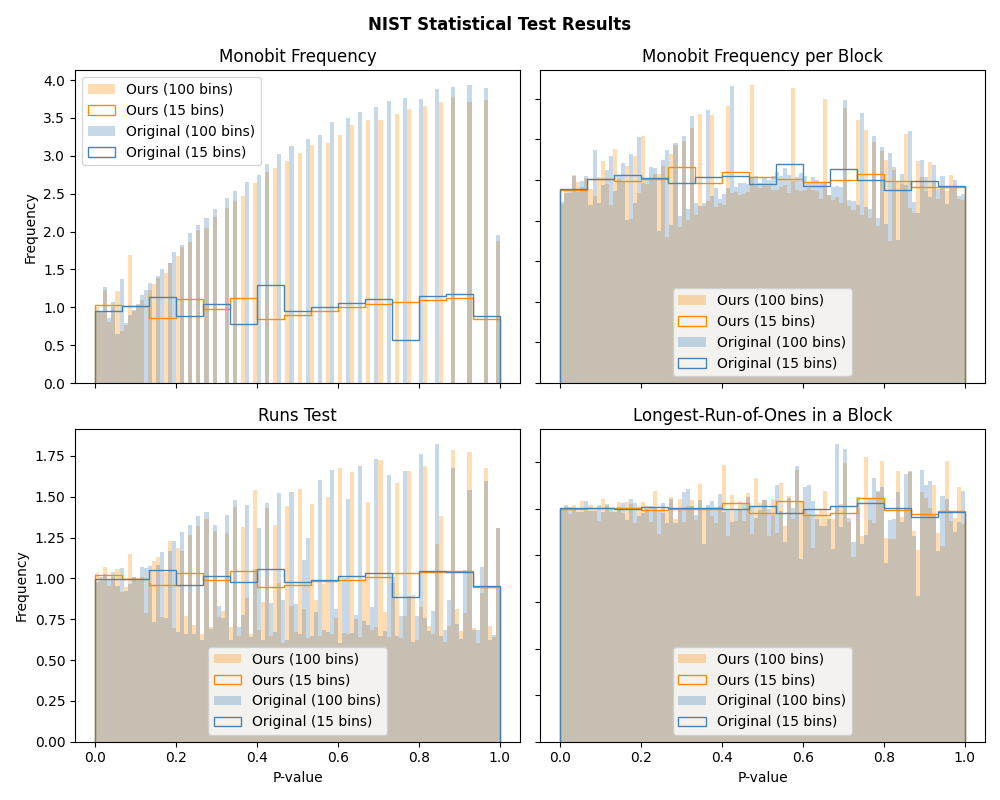
\includegraphics[width=0.9\linewidth]{Images/25-05-19-runwise_comparison_400000h-20n-3m-3p5.png}
    \caption{Distribution of NIST SP 800-22 p-values across 400 000 headers (headerwise evaluation).}
    \label{fig:sp_800-22_hist_headerwise}
\end{figure}
\begin{figure}[H]
    \centering
    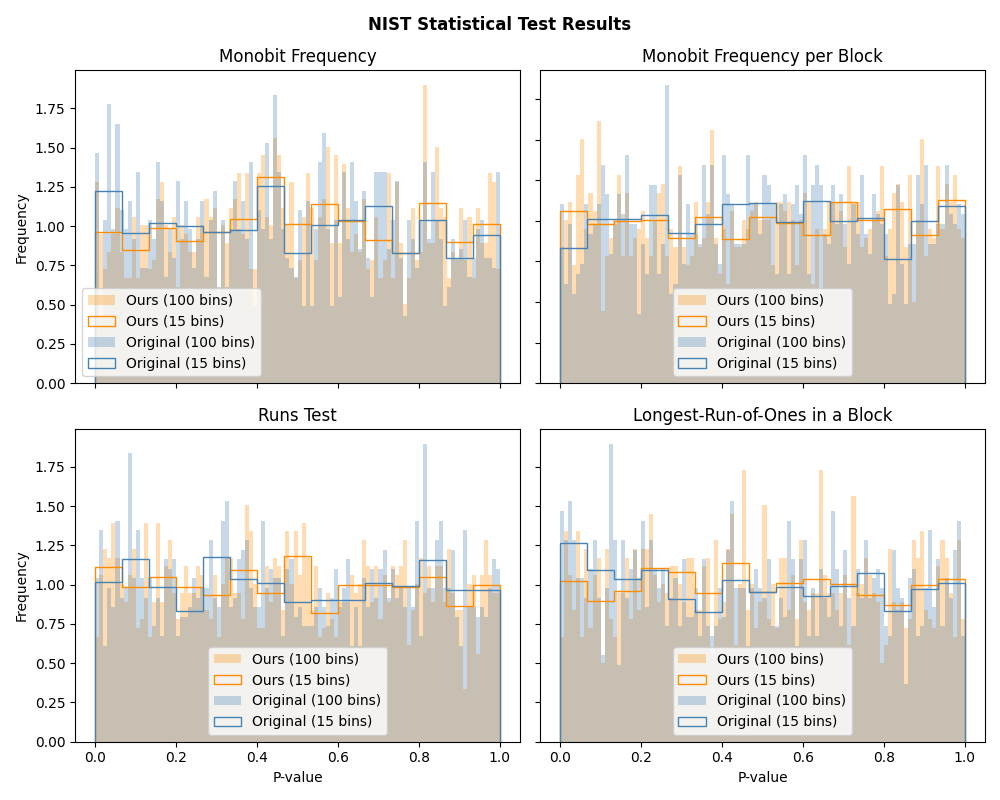
\includegraphics[width=0.9\linewidth]{Images/25-05-19-bitwise_comparison_400000h-20n-3m-3p5.png}
    \caption{Distribution of NIST SP 800-22 p-values per bit across 400 000 headers (bitwise evaluation).}
    \label{fig:sp_800-22_hist_bitwise}
\end{figure}

Some deviations in the histograms arise from the limited size of the bitstrings (1634 or 1792 bits), which introduces quantization effects. 
In particular, the slight distortion in the first test of Figure \ref{fig:sp_800-22_hist_headerwise} reflects the granularity of possible p-values for short inputs. 
Variations in Figure \ref{fig:sp_800-22_hist_bitwise} are due to the small amount of p-values (1634 or 1792).
Increasing the histogram bin size mitigates these artifacts and confirms that the underlying distributions remain approximately uniform.

In both evaluations, the distributions of p-values are approximately uniform, which suggests that headers are statistically indistinguishable from random data, 
and therefore indicates strong linkability resistance, comparable to the original Sphinx implementation.
